\documentclass[a4paper,11pt]{article}
\usepackage[utf8]{inputenc}
\usepackage[T1]{fontenc}
\usepackage[french]{babel}
\usepackage{makeidx}
\usepackage{textcomp}
\usepackage{graphicx}
\usepackage{mathtools,amssymb,amsthm}
\usepackage{lmodern}
\usepackage{multirow}
\usepackage{array}
\usepackage{longtable}

\title{TER 2019 - Rapport}
\author{Maxime Gonthier - Benjamin Guillot - Laureline Martin}
\begin{document}
\pagenumbering{gobble}\clearpage
\maketitle

\newpage
\tableofcontents

\newpage
\section{Introduction}
	Ce rapport a pour objectif de décrire dans un premier temps les données que nous allons utiliser dans notre projet, nous détaillerons les étapes à suivre pour exploiter ces données. Dans un second temps nous expliquerons le calcul de la congestion. Enfin nous expliquerons la stratégie d'optimisations que nous utiliserons. Tous cela sera expliciter sous la forme d'un exemple simple.

\section{Les données initiales}
	\subsection{La courbe de trafic}
		La courbe de trafic représente le nombre de personnes qui montent et descendent du bus à chaque arrêt. Dans notre cas d'étude, nous considérons que tous les étudiants montent au premier arrêt (gare des chantiers) et descendent au terminus (l'université). La courbe de trafic est aussi composée des montées et des descentes à chaque arrêt de personnes non-étudiants. \\
		Dans notre exemple nous avons : \\
		\begin{tabular}{ | c | c | c | c | c | c |}
 			\hline			
   			Numéro de l'arrêt	& 1 	& 2 	& 3 	& 4 	& 5\\
   			montées				& 50 	& 15 	& 10 	& 2 	& 0\\
   			Descentes			& 0 	& 5 	& 10 	& 8 	& 54\\
 			\hline  
 		\end{tabular}\\
 		La valeur de montée des non-étudiants au premier arrêt est composée .
 		Pour obtenir les données des arrêts intermédiaires nous choisirons une valeur aléatoire, choisis dans un intervalle différent en fonction de l'heure, l'objectif est de représenter la congestion forte des heures de pointes de manière un peu plus précise : \\
 		\begin{tabular}{ | c | c | c | c | c | c | c | c | c | c |}
 			\hline			
   			Horaire & 7-8h & 8-9h & 9-10h & 10-11h & 11-12h & 12-13h & 13-14h & 14-15h & 15-16h\\
   			Montées & [5:15] & [5:15] & [3:10] & [2:8] & [1:5] & [1:5] & [1:5] & [2:8] & [3:10]\\
   			Descentes & [0:5] & [0:5] & [1:6] & [1:6] & [1:5] & [1:5] & [0:5] & [0:5] & [1:5]\\
 			\hline  
 		\end{tabular}\\

	\subsection{L'emploi du temps}
		L'emploi du temps est un graphe dont les sommets sont des cours et les liens des contraintes entre les cours.
		Pour plus de clarté nous considérons ici que chaque professeur est disponible sur toute la durée de la journée.
		Dans notre exemple nous nous limitons à 10 sommets.
		\begin{enumerate}
			\item On créer un graphe non orienté en numérotant les sommets de 1 à 10.
			\centerline{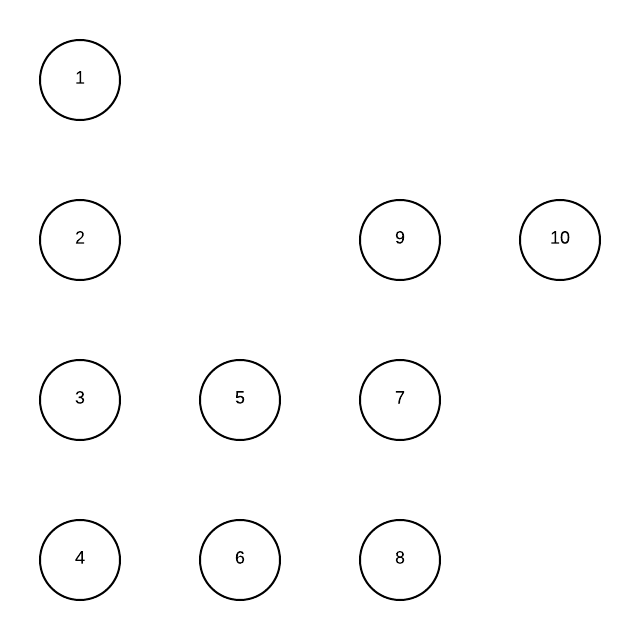
\includegraphics[scale=0.8]{Captures/exemple1.png}}
			\item On relie les sommets entre eux lorsque qu'il y a une contrainte (même étudiant sur des horaires qui se chevauchent). Pour cela on créé une matrice d'adjacence avec un degré moyen choisis arbitrairement. Pour N sommets et K le degré moyen, la probabilité qu'ily ai une arête à insérer dans chaque case est K/N.
			\item On oriente les arêtes désormais des arcs du plus faible au plus fort
			\centerline{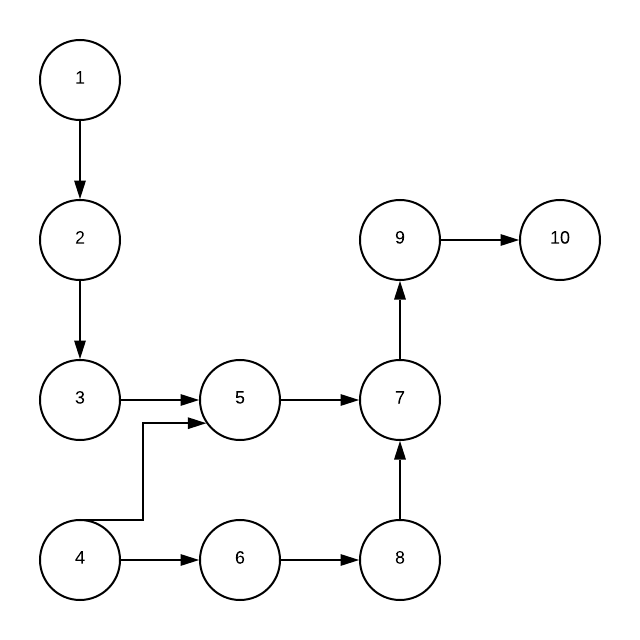
\includegraphics[scale=0.8]{Captures/exemple2.png}}
			\item On remarque dans notre exemple qu'il y a deux sommets de degré entrant nul, ces deux sommets de notre DAG seront des points de départs possible pour notre planification.
			\item On colorie le graphe, chaque couleur représente une salle.\\
			\centerline{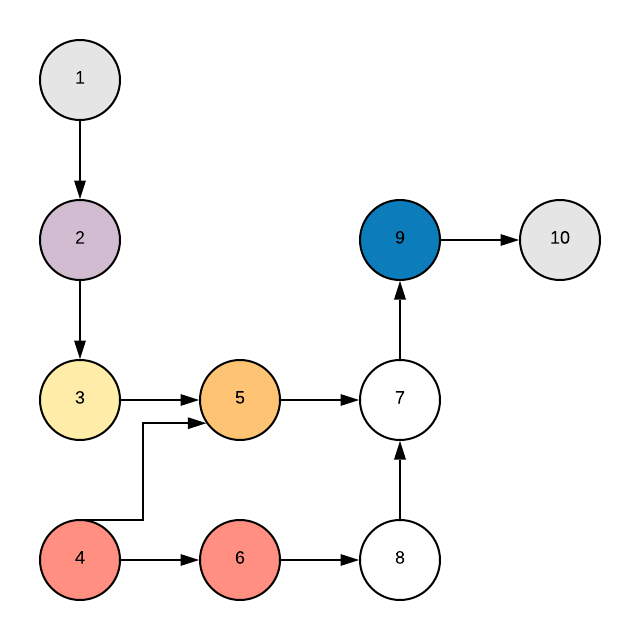
\includegraphics[scale=0.8]{Captures/exemple3.png}}
			\item Nous agencons l'emploi du temps en respectant le fait que deux couleurs et deux sommets reliés par un arc ne peuvent pas être sur la même plage horaire. Par défaut le sommet duquel nous partirons est le sommet de degré entrant nul le plus faible, ici le numéro 1.
			\centerline{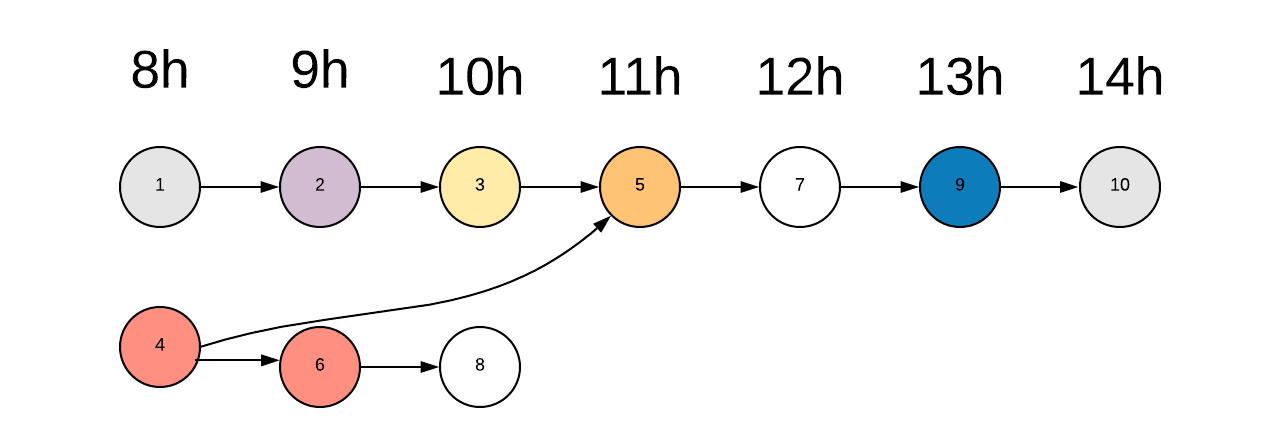
\includegraphics[scale=0.8]{Captures/exemple4.png}}
		\end{enumerate}
		Chaque cours possède un nombre d'étudiants choisis aléatoirement entre 16 et 32 pour un TD et entre 16 et 100 pour un cours magistral. les TDs représentent trois quart des cours. Ainsi dans notre exemple nous avons : \\
		\begin{tabular}{ | c | c | c | c | c | c | c | c | c | c | c |}
 			\hline			
   			Numéro du sommet & 1 & 2 & 3 & 4 & 5 & 6 & 7 & 8 & 9 & 10\\
   			Type de cour & TD & CM & CM & TD & TD & TD & TD & TD & TD & CM \\
   			Nombre d'élèves & 16 & 70 & 60 & 30 & 25 & 20 & 16 & 30 & 14 & 50\\
 			\hline  
 		\end{tabular}\\

\section{Calcul de congestion}
	A l'aide du tableau ci dessus nous allons pouvoir déterminé à chaque horaire le nombre d'étudiants arrivé au terminus et donc en conclure à l'aide du tableau des montées et des descentes le nombre de personnes à chaque arrêt. 
	On considère que les etudiants prennent le bus arrivant 15 min avant leurs premier cour de la journée.
	Dans notre exemple nous avons pour  8h le cours 1 et 4, ce qui représente 46 élèves. Ainsi le bus de arrivant a 7h45 ressemble à cela :  \\
	\begin{tabular}{ | c | c | c | c | c | c | c |}
 			\hline			
   			Numéro de l'arrêt & 1 & 2 & 3 & 4 & 5\\
   			Différence montées/descentes & 10 & 7 & 10 & 11 & 0\\
   			Nombre de personnes dans le bus & 56 & 53 & 60 & 56 & 57\\
 			\hline  
 	\end{tabular}\\
 	Ce tableau sera générés pour chaque bus. On mesurera dans chaque cas le dépassement à chaque arrêt en mettant un 1 si il y a dépassements, un 0 sinon.
 	Sachant que la limite de confort est de 50 dans le bus que nous étudions, ce bus nous donne une valeur de congestion de 5.
 	Il faudra pour les bus suivants prendre en compte les élèves déjà présent à l'université avant de calculer le nombre de personnes dans le bus.

\section{Stratégie d'optimisation}
	\subsection{Mise en rapport de la congestion et des sommets}
		Il faut dans un premier temps déterminer quels sommets sont les plus impactant en terme de congestion. Une manière de les trier peut être par ordre décroissant de leurs nombre d'étudiants. Ensuite on rechercherais une solution gloutonne où les sommets ayant le plus d'étudiants ont lieu à des horaires où les autres cours ont peu d'étudiants, c'est à dire que nous allons minimiser la somme des étudiants ayant cours au même moments. Si il y a un choix à faire on place le cours avec le plus d'étudiant sur l'horaire où la congestion des non-étudiants est la plus faible (c'est à dire s'éloigner de l'horaire 7:8h. Evidemment le point de départ sera toujours un sommet de degré entrant nul. Dans notre exemple on aurait pour le tri : \\
		\begin{tabular}{ | c | c | c | c | c | c | c | c | c | c | c |}
 			\hline			
   			Numéro du sommet & 2 & 3 & 10 & 4 & 8 & 5 & 6 & 7 & 1 & 9\\
   			Nombre d'élèves & 70 & 60 & 50 & 30 & 30 & 25 & 20 & 16 & 16 & 14\\
 			\hline  
 		\end{tabular}\\	
 		On place en premier le sommet 1 à 8h car il a moins d'étudiants que le 4 et que nous avons décider d'éloigner les cours chargées des horaires de congestions des non-étudiants en cas de conflits.. Ensuite on place le sommet 2 à 9h pour ne pas être en même temps que le 4. Ainsi de suite. Une fois arrivé à l'horaire limite de notre exemple (14h) on place les sommets au endroit où la somme des étudiants sera le plus faible possible. Ainsi le sommet 6 va à la même horaire que le sommet 5, le 7 à la même horaire que le 8, impossible ils ont la même couleur, donc le 7 va a la même horaire que le suivant, le 4 etc...
 		Après l'optimisation gloutonne on aura : \\
 		\centerline{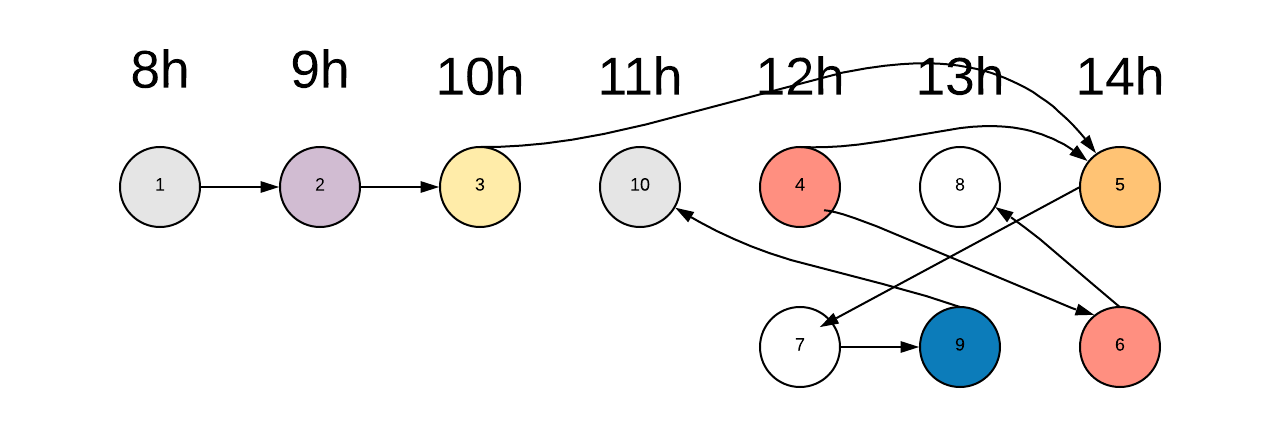
\includegraphics[scale=0.8]{Captures/exemple5.png}}\\
 		On reclacule ensuite la congestion de chaque bus comme vue précedemment.

 	\subsection{Recherche tabou}
 		A partir de la première solution obtenu grace à l'approche gloutonne nous allons explorer le voisinage de cette dernière pour tenter de trouver des optimums locaux.\\
 		On va modifier l'horaire des cours 1 à 1 de manière aléatoire en commencant par le cours ayant le plus d'étudiant. Pour chaque solution on recalcule la congestion et on interdit la configuration pour les prochaines solutions. Dans notre exemple on va dans un premier temps bouger le sommet 2 de 9h à 10h. Ensuite on recherche la solution suivante en prenant en compte cette modification. On procède de la sorte pendant un nombre d'itérations arbitraire. En effet on ne peux pas savoir quand arrêter la simulation car on ne peux pas être sûr qu'un optimum local est aussi global.\\
 		Ensuite nous allons appliquer le même procéder mais en faisant varier les horaires deux sommets à la fois a chaque itérations.
 		A MIEUX ECRIRE / RAJOUTER DES CHOSES
\end{document}
